\underline{Sieć Hopfielda} jest przykładem sieci ze sprzężeniem zwrotnym (tzw. sieć rekurencyjna), gdzie wyjścia poszczególnych neuronów są podawane z odpowiednimi wagami na wejścia każdego z neuronów. Oczywiście do każdego neuronu podpięte jest wejście, którym doprowadzana jest odpowiednia składowa wektora testowego. Założenia:
\begin{itemize}
	\item całkowite połącznie neuronów,
	\item neurony 2-stanowe,
	\item symetryczne połączenia synaptyczne
	\item synchroniczna dynamika sieci
\end{itemize}

\begin{figure} [H]
	\centering
	\begin{subfigure}{.69\textwidth}
		\centering
		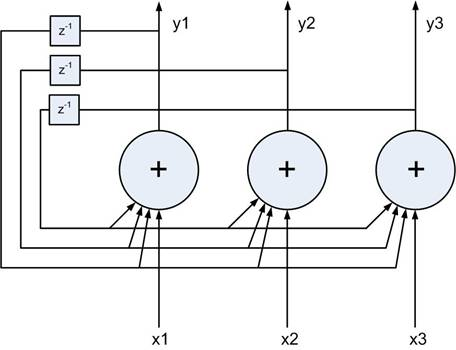
\includegraphics[width=1.0\linewidth]{EDMIIssues/Figures/hopfield.jpg}
	\end{subfigure}
	\caption{Równania Maxwella.}
	\label{hopfield}
\end{figure}

W sieciach Hopfielda waga połączenia wyjścia neuronu z własnym wejściem jest zerowana. Wymagane jest także, aby macierz wag $ W $ była symetryczna.

Funkcja aktywacji pojedynczego neuronu wygląda następująco:\newline
$ y_i(t+1) = 1 $, gdy $ \sum_{j=1}^N w_{ij}y_j(t) + x_i(t) + \xi_i(t) > 0 $,]\newline
$ y_i(t+1) = y_i(t) $, gdy $ \sum_{j=1}^N w_{ij}y_j(t) + x_i(t) + \xi_i(t) = 0 $,\newline
$ y_i(t+1) = -1 $, gdy $ \sum_{j=1}^N w_{ij}y_j(t) + x_i(t) + \xi_i(t) < 0 $, gdzie:\newline
$ i $ oraz $ j $ oznaczają numery neuronów $ N $-neuronowej sieci Hopfielda, $ \xi $ oznacza szum (np. gaussowski o $ \mu $ = 0),  natomiast $ t $ przedstawia chwilę czasową. Należy również zwrócić uwagę na to, że składowe wektora $ x $ w chwili czasowej $ t=0 $ są przepisywane na wyjścia neuronów, natomiast dla $ t>0 $ wejścia są „odpinane” od neuronów ($ x=0 $).

W trybie uczenia, na podstawie zbioru wektorów uczących obliczane są wagi. Najprostszą metodą (wykorzystywaną w naszym przykładzie) uczenia sieci jest reguła Hebb’a. Wagi obliczane są według wzoru:\newline
$ w_{ij} = \dfrac{1}{N} \sum_{k=1}^K x_i^{(k)}x_j^{(k)} $, gdzie $ k $ oznacza numer wektora uczącego, a $ K $ liczbę wszystkich wektorów uczących.

Okazuje się, że gdy na wejście sieci podamy wektor identyczny z wzorcem, wówczas sieć nie zmieni swojego stanu, rozpoznaje ona również obrazy „niewiele” różniące się od wzorców. W niektórych przypadkach pojawia się kolejna cecha sieci Hopfielda - pamiętanie zależności pomiędzy sąsiednimi pikselami, a nie ich wartości. Wtedy otrzymujemy obraz wzorca z odwróconymi kolorami.

Miara podobieństwa wzorca $ k $-tego (pokrycie ang. \textit{overlap}):\newline
$ m^k(t) = \dfrac{1}{N} \sum_{i=1}^{N} y_i(t)x^{(k)}_i $.

Gdy:\newline
$ m^k = 1 $ - całkowita zgodność wzorca,\newline
$ m^k = 0 $ - całkowita niezgodność wzorca,\newline
$ m^k = -1 $ - stan sieci jest negatywem wzorca.

Sieć Hopfielda jest ograniczona ilością wzorców, które może zapamiętać i skutecznie rozróżniać. Jeśli $ p $ - ilość zapamiętanych wzorców, a $ N \to \infty $ - liczba neuronów, to $ p_c = \dfrac{p}{N} \approx 0,138 $, przy założeniu, że średnie pokrycie wzorców nie spada poniżej 95\%.

Liczbę identycznych bitów w dwóch stanach sieci nazywamy odległością Hamminga. Proces ewaluacji wzorca wejściowego zatrzymujemy, gdy wrzozec wyjściowy zbliży się na pewną, ustaloną odległość Hamminga do któregoś z zapamiętanych wzorców.


